\chapter{提案手法}
\thispagestyle{fancy}

\section{使用装置}
\subsection{Kinect for Windows}
Microsoftから販売された,コントローラーを用いずに身体の動き,ジェスチャー,音声などによって
操作を可能にする周辺機器である.

Kinectには,赤外線センサー,8ビット3チャンネル(RGB)の画像データを取得するRGBカメラ,
Kinectからの距離(深度)の画像データを取得する深度画像センサー,音の発生場所を求める
音源位置推定が可能な音声マイクが搭載されている.
また,Kinectの最も特徴的な機能が「姿勢認識技術」である,人間の全身を認識してその動きによる操作をしている.
これにより,深度画像をもとに,人体のパーツがどこにあるのかを推測することができる\cite{kinect}.

本研究では,Kinect for Windows v1を使用した.

\begin{figure}[b]
    \centering
    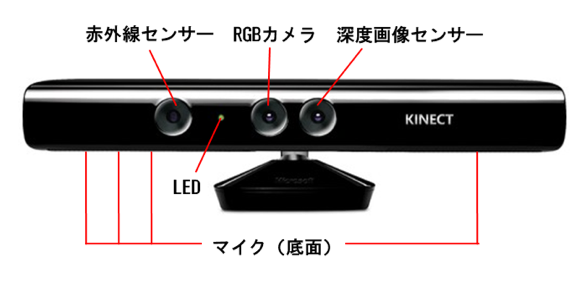
\includegraphics[width=9cm]{image/kinect.png}
    \caption{Kinect for Windows\cite{kinect}}
  \label{kinect}
\end{figure}

\clearpage

\subsection{プロジェクター}
投影を行う際に使用した.


\section{開発環境}

\begin{itemize}
    \item OS: Windows 10
    \item 統合開発環境: Visual Studio 2017
    \item プログラミング言語: C++
    \item ライブラリ: OpenNI2, NiTE2, OpenCV, OpenGL
\end{itemize}

\section{システムの概要}
本研究では,スポーツに焦点を当て野球とサッカーのアクションを行えるプロジェクションマッピングを実装した.


\subsection{骨格座標を用いた手法}
\subsubsection{表示画面}
\label{kokkaku}
以下の7つの画面を出力する.

\begin{itemize}
    \item Ball: スポーツで用いるボール.図\ref{ball}.
    \item Color: RGBカメラの映像.図\ref{color}.
    \item Depth: 深度カメラの映像.図\ref{depth}.
    \item User: 人領域の映像.図\ref{user}.
    \item Combination: 投影用.図\ref{combination}.
    \item Combination\_PC: PC用.図\ref{combination}.
    \item Skeleton: 人の骨格情報.図\ref{skeleton}.
\end{itemize}

\clearpage

\begin{figure}[p]
    \begin{minipage}{0.5\hsize}
     \begin{center}
      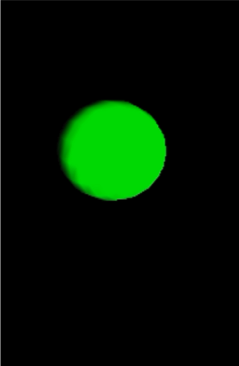
\includegraphics[width=4cm,height=6cm]{image/ball.png}
     \end{center}
     \caption{Ballの画面表示}
     \label{ball}
    \end{minipage}
    \begin{minipage}{0.5\hsize}
     \begin{center}
      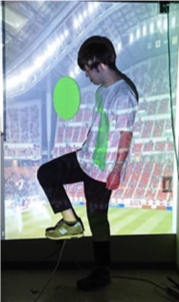
\includegraphics[width=4cm,height=6cm]{image/color.png}
     \end{center}
     \caption{Colorの画面表示}
     \label{color}
    \end{minipage}
\end{figure}

\begin{figure}[p]
    \begin{minipage}{0.5\hsize}
     \begin{center}
      \includegraphics[width=4cm,height=6cm]{image/Depth.png}
     \end{center}
     \caption{Depthの画面表示}
     \label{depth}
    \end{minipage}
    \begin{minipage}{0.5\hsize}
     \begin{center}
      \includegraphics[width=4cm,height=6cm]{image/User.png}
     \end{center}
     \caption{Userの画面表示}
     \label{user}
    \end{minipage}
\end{figure}

\clearpage

\begin{figure}[p]
    \begin{minipage}{0.5\hsize}
     \begin{center}
      \includegraphics[width=4cm,height=6cm]{image/Combination.png}
     \end{center}
     \caption{CombinationとCombination\_PCの画面表示}
     \label{combination}
    \end{minipage}
    \begin{minipage}{0.5\hsize}
     \begin{center}
      \includegraphics[width=4cm,height=6cm]{image/Skeleton.png}
     \end{center}
     \caption{Skeletonの画面表示}
     \label{skeleton}
    \end{minipage}
\end{figure}

\clearpage

\subsubsection{スケルトンナンバーについて}
Kinect v1において,スケルトンは図\ref{num}に示すように番号が割り当てられている.

\begin{figure}[htbp]
    \centering
    \includegraphics[height=7cm]{image/Skeleton_num.png}
    \caption{スケルトンナンバー}
  \label{num}
\end{figure}

\begin{table}[h]
    \centering
    \begin{tabular}{|lc|lc|} \hline
      0 & 頭 & 8 & 胴体 \\ 
      1 & 首 & 9 & 左腰 \\
      2 & 左肩 & 10 & 右腰 \\
      3 & 右肩 & 11 & 左膝 \\
      4 & 左肘 & 12 & 右膝 \\
      5 & 右肘 & 13 & 左足 \\
      6 & 左手 & 14 & 右足 \\
      7 & 右手 &  &  \\ \hline
    \end{tabular}
    \caption{スケルトンナンバーと体の位置関係}
    \label{num}
\end{table}

\clearpage
\subsubsection{手法}
ユーザにCombination画面の投影を行い,ユーザのスケルトン座標に応じてインタラクティブに
プロジェクションマッピングが変化する.
システム起動時,スケルトンの認識が不安定となるため,意図していないモードに切り替わる場合がある.
それを防ぐために「気を付け」のポーズをとる.このポーズは,左肩と右肩の$y$座標の差が$100mm$未満,
かつ左肘と右肘の$y$座標の差が$150mm$未満の場合に対応している(図\ref{num}参照).
モードの一連の動作が終了すると,初期化される.そのため,連続して投影を行うことが可能となる.
それぞれのモードに切り替わる前は,画面は黒いままである.

\subsubsection{野球モード}
ピッチャーの一連の動作を行うと,野球ボールと野球場が投影される.
ボールは投げる際に音がなり,飛距離が伸びるにつれ,徐々に小さくなるようにしている.
ボールの位置が$x$座標のしきい値(被験者から見て画面左端)より大きくなった場合,ボールは消えて初期化される.

以下にその手順を示す.

\begin{enumerate}
    \item 胸の付近で両手を構える(以下の6つの条件を満たす必要がある)
        \begin{itemize}
            \item 左肘の$x$座標と胴の中心の$x$座標の差が$180mm$未満
            \item 左肘の$y$座標と胴の中心の$y$座標の差が$180mm$未満
            \item 右肘の$x$座標と胴の中心の$x$座標の差が$180mm$未満
            \item 右肘の$y$座標と胴の中心の$y$座標の差が$180mm$未満
            \item 首の$y$座標と左手の$y$座標の差が$180mm$未満
            \item 首の$y$座標と右手の$y$座標の差が$180mm$未満
        \end{itemize}
    \item 頭より上に来るように右手を振り上げるとボールが出現し動き出す(以下の条件で認識する).
        \begin{itemize}
            \item 振り上げた右手の$y$座標が頭の中心の$y$座標よりも高い
        \end{itemize}
\end{enumerate}

\clearpage

\begin{figure}[t]
    \centering
    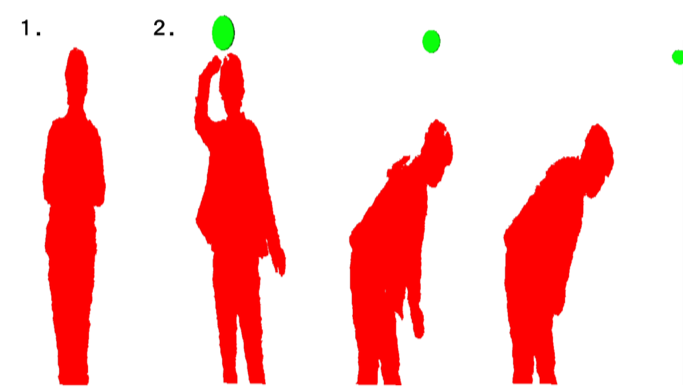
\includegraphics[width=8cm]{image/baseball.png}
    \caption{野球モードを実行した際のCombinationの画面表示}
  \label{baseball}
\end{figure}


\subsubsection{サッカーモード}
リフティングの一連の動作を行うと,サッカーボールとサッカー場が投影される.
ボールを蹴り上げる際には音がなる.また,
ボールの位置が$y$座標のしきい値(画面下)より低くなった場合,ボールは消え初期化される.

以下にその手順を示す.

\begin{enumerate}
    \item 右膝を右腰ほどの高さになるように蹴り上げるとボールが出現する(以下の条件で認識する).
        \begin{itemize}
            \item 右膝の$y$座標が右腰から$300mm$低い位置より高く蹴り上げると,ボールが出現し動き出す.            
        \end{itemize}
    \item 右膝を下ろすとボールは下がり続ける.
\end{enumerate}


\begin{figure}[b]
    \centering
    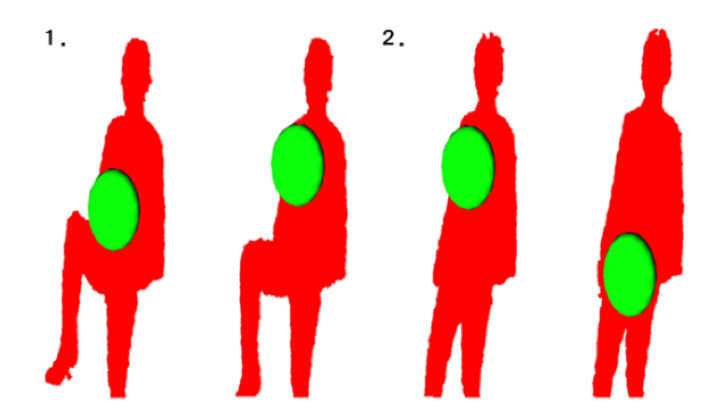
\includegraphics[width=8cm]{image/soccer.png}
    \caption{サッカーモードを実行した際のCombinationの画面表示}
  \label{baseball}
\end{figure}

\clearpage

また,リフティングの動きは,以下の物理演算を使用している.

$y$座標は上向きを正とし,プロジェクションマッピングの画面中央を$y=0$とする.



\begin{figure}[htbp]
    \centering
    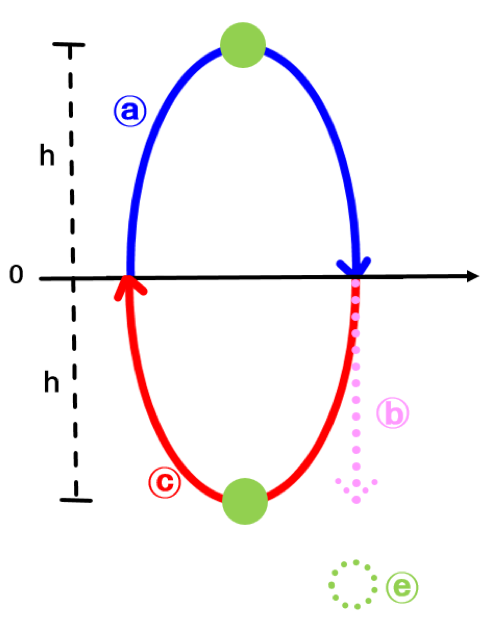
\includegraphics[width=7cm]{image/butsuri.png}
    \caption{リフティングの動きを実装するために使用した物理演算}
  \label{butsuri}
\end{figure}



\[
    \begin{cases}
        v_0,v_0': 初速度 & \\
        t: 時間 & \\
        g: 重力加速度(g=9.8)とする. &
    \end{cases}
\]

\vspace{1cm}

\begin{itemize}
    \item[a] ボールの位置が$y \geqq 0$の場合
        \begin{equation}
            y=v_0t-\frac{1}{2}gt^2
        \end{equation}
        \begin{equation}
            v_0=25とすると,y=25*t-\frac{1}{2}gt^2
        \end{equation}
        
    \item[bc] ボールの位置が$y < 0$の場合
        \begin{itemize}
            \item[b] 一定速度で落下
            \item[c] ボールを蹴り上げる動作をした時
                \begin{equation}
                    y=v_0't-\frac{1}{2}gt^2
                \end{equation}
        \end{itemize}
\end{itemize}

\begin{figure}[htbp]
    \centering
    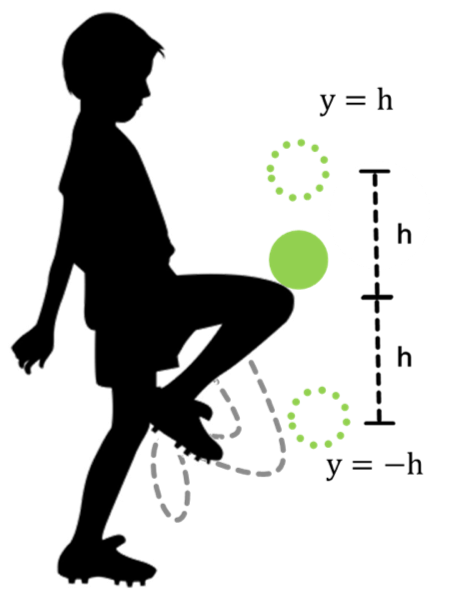
\includegraphics[width=6cm]{image/ballenzan.png}
    \caption{ボールを蹴り上げた時点でのボールの位置}
  \label{enzan}
\end{figure}

\vspace{1cm}

ボールの最高点の位置を$y=h$(図\ref{butsuri}参照)

ボールを蹴り上げた時点でのボールの位置を$y=-h$(図\ref{butsuri},図\ref{enzan}参照)
と仮定する.

連続したリフティング動作を行えるようにするため,aでのボールの最高点に,
再び蹴り上げたボールの高さをそろえる.これを実現させるため,以下の計算を行う(図\ref{butsuri}参照).


\begin{itemize}
    \item[aより]
        \begin{equation}
            v^2-v_0^2=2(-g)h
        \end{equation}

        最高点の速さは$v=0$より 

        \begin{equation}
            0-v_2^2=2(-g)h
        \end{equation}
\clearpage
        よって

        \begin{equation}
            v_0=\sqrt{2gh}
        \end{equation}

    \item[cより]
        \begin{equation}
            v^2-v_0'^2=2(-g)(2h)
        \end{equation}

        最高点の速さは$v=0$より 

        \begin{equation}
            0-v_0'^2=2(-g)(2h)
        \end{equation}
        よって

        \begin{equation}
            v_0'=\sqrt{4gh}
        \end{equation}

    \item[以上より]
        \begin{equation}
            v_0'=\sqrt{2}v_0
        \end{equation}

        よって$v_0'$は$v_0$の$\sqrt{2}$倍である. 

        \begin{equation}
            v_0'=25*\sqrt{2} \fallingdotseq 35.4 
        \end{equation}

        より

        \begin{equation}
            y=35.4*t-\frac{1}{2}gt^2
        \end{equation}

    \item[dより] ボールが閾値(画面下)より低くなった場合ボールは消える. 

\end{itemize}


\clearpage
\subsection{物体検出器を用いた手法}
\subsubsection{表示画面}
節\ref{kokkaku}の骨格座標を用いた手法の表示画面にさらに以下の2つ画面を追加した.